% this file is called up by thesis.tex
% content in this file will be fed into the main document

% change according to folder and file names
\ifpdf
    \graphicspath{{figures/}{figures/comparisons}}
\else
    \graphicspath{{figures/}{figures/comparisons}}
\fi

\chapter{Structure From Motion with Sensor Fusion} \label{chap:structure_from_motion}
All implemented algorithms were tested in terms of speed, accuracy and effectiveness. As regards the speed test, it included the measurement of the reconstruction execution time. In the accuracy testing Sampson Error measurement was used (this variable measures the distance between all points and their corresponding epipolar lines in an image). Effectiveness was tested with the use of the visual comparison of reconstructed 3D cloud points.
\section{Concept}
\subsection{Reconstruction process strategy}
Finally, all methods described herein can be combined in different reconstruction strategies. For the initialisation of 3D cloud point the following strategies can be used:
\begin{enumerate} 
\item \textbf{Known rotations and translations}, which theoretically allows for an metrical reconstruction
\item \textbf{Known rotations}, where translation is estimated with an alternative 3-point algorithm
\item \textbf{Noisy rotations}, where enhanced 8-point fundamental or 5-point essential algorithms are used in order to calculate rotation error and relative translation 
\item \textbf{Unknown external camera parameters}, where standard 8-point fundamental or 5-point essential algorithms are used in order to calculate rotation and relative translation
\end{enumerate}
For the pose estimation the following methodologies can be used:
\begin{enumerate}
\item \textbf{Known rotations and translations}, where no additional calculations are required and an metrical model can be acquired
\item \textbf{Initial rotation}, where relative translation needs to be calculated
\item \textbf{Noisy rotation and translation}, where both rotation and translation errors need to be calculated
\item \textbf{Unknown external camera parameters}, where standard pose estimation has to be used
\end{enumerate}
All proposed strategies were implemented and can be tested in desktop Application.

\subsection{Pose estimation}
One of the main goal was to develop a more accurate and faster version of the reconstruction algorithm. That is why the relative pose estimation techniques were used to enrich models with additional points. In general, this approach produces less outliers than the homography merging techniques. This also allows to maintain the scale of the reconstructed images. For any point of the image, which has a corresponding 3D point the following condition is met:
\begin{equation} \label{eq:projectionEquation}
 x = P * X
\end{equation}
where x is image point expressed in homogenous coordinates (x , y , 1) and X homogenous 3D point (X , Y , Z , 1). 
The projection matrix of the camera design is as follows: 
\begin{equation} \label{eq:projectionEquation}
 P = K * \begin{bmatrix}R\mid t\end{bmatrix}
\end{equation}
\subsubsection{Rotation enhancements}
Applying the similar approach to initial pair reconstruction enhancements, it can be noted that:
\begin{equation} \label{eq:projectionRotError1}
\begin{array}{rcl}
 x & = & K * \begin{bmatrix}R_{init} + dR\mid t\end{bmatrix} * X \\
 x & = & K * \begin{bmatrix}T_{init}\mid 0\end{bmatrix} * X + K * \begin{bmatrix}dR\mid t\end{bmatrix} * X \\
 x - K * \begin{bmatrix}R_{init}\mid 0\end{bmatrix} & = & K * \begin{bmatrix}dR\mid t\end{bmatrix} * X
\end{array}
\end{equation}
Substituting $x_{m} = x - K * \begin{bmatrix}R_{init}\mid 0\end{bmatrix}$ the following is received: 
\begin{equation} \label{eq:projectionRotError2}
x_{m} = K * \begin{bmatrix}dR\mid t\end{bmatrix} * X
\end{equation}
This can be solved using a standard PNP calculating algorithms. Rotation can be used as an initial solution for the pose estimation in order to focus solely on the rotation error and translation estimation.
\subsubsection{Rotation \& translation enhancements}
Similar to equation \ref{eq:projectionRotError1}:
\begin{equation} \label{eq:projectionRotError3}
\begin{array}{rcl}
 x & = & K * \begin{bmatrix}R_{init} + dR\mid T_{init} + dt\end{bmatrix} * X \\
 x & = & K * \begin{bmatrix}R_{init}\mid T_{init}\end{bmatrix} * X + K * \begin{bmatrix}dR\mid dt\end{bmatrix} * X \\
 x - K * \begin{bmatrix}R_{init}\mid T_{init}\end{bmatrix} & = & K * \begin{bmatrix}dR\mid dt\end{bmatrix} * X
\end{array}
\end{equation}
end in the end by substituting $x_{n} = x - K * \begin{bmatrix}R_{init}\mid T_{init}\end{bmatrix}$ the following is received: 
\begin{equation} \label{eq:projectionRotError4}
x_{n} = K * \begin{bmatrix}dR\mid dt\end{bmatrix} * X
\end{equation}
This can also be solved using a standard PNP\cite{website:poseEstimation} calculation algorithm. Rotation and translation can be used as an initial solution for the pose estimation in order to focus solely on the rotation error and translation error estimation.

\ifpdf
    \graphicspath{{figures/}{figures/comparisons}}
\else
    \graphicspath{{figures/}{figures/comparisons}}
\fi

%: ----------------------- name of chapter  -------------------------
\section{Implementation} % top level followed by section, subsection
This chapter describes the chosen implementation environment. It also describes an Android application which was created for the purpose of acquiring image sequences with additional sensor data. The structure of both Android and desktop projects is explained and essential implementation details of the proposed algorithms and strategies are discussed herein.

\subsection{Enhancing pose estimation}
OpenCV already has the rotation and translation enhanced pose estimation implemented. The only thing that has to be done is the conversion of euclidean rotation matrix to its Rodrigues representation. The initial rotation and translation need to be passed as input variables. Pose estimation methods implementations are as follows: 
\begin{lstlisting}
Mutiview::FindPoseEstimation(
        cv::Mat &rvec,
        cv::Mat &t,
        cv::Mat &R,
        cv::Mat &K,
        cv::Mat &distCoeffs,
        std::vector<cv::Point3d> ppcloud,
        std::vector<cv::Point2d> imgPoints,
        vector<int> inliers) 
Mutiview::FindPoseEstimationEnhanced(
        cv::Mat &rvec,
        cv::Mat &t,
        cv::Mat &R,
        cv::Mat &RInit,
        cv::Mat &TInit,
        cv::Mat &K,
        cv::Mat &distCoeffs,
        std::vector<cv::Point3d> ppcloud,
        std::vector<cv::Point2d> imgPoints,
        vector<int> inliers)
\end{lstlisting}
can be found in 'Mutiview.cpp' file.


% ----------------------- contents from here ------------------------
\section{Evaluation}
\subsection{Acquiring datasets}
For the purpose of analysis the following datasets were captured with the implemented ''Sensor Enhanced Images Camera'' application and Nexus 5 camera:
\begin{enumerate}
\item Warsaw University of technology main building
\item Advertisement Pole 
\item Warsaw Business School Gate and Entrance
\item Warsaw Shopping Center Back
\item Warsaw Shopping Center Front
\end{enumerate}
Since most of the algorithms proposed in the Chapter 4 require internal camera parameters to be known, the camera used in the course of conducting this study was calibrated and its parameters were stored in \textit{''outcameradata.yml''} file. All of these datasets can be found on attached CD or in Github repository.
\subsection{Test Environment}
All tests were performed on MacBook Air with 1.7GHz dual-core Intel Core i7 processor and 8GB 1600MHz DDR3 RAM using ''Enhanced 3D Reconstructer'' implemented as described in the Implementation chapter.  Numerical tests which allowed for measuring total errors and execution time were run on the ''Warsaw University of Technology'' dataset. Initial pair reconstruction ability of each method proposed was measured as well as various reconstruction strategies.  Finally, for each dataset the most effective methods were used to reconstruct sparse models. 
\subsection{Testing initial pair reconstruction methods} \label{sec:Testin2Views}
The key question to be answered at this point was whether the proposed sensor enhancement gave better results than the standard algorithms.
The following methods were tested:
\begin{enumerate}
\item \textbf{Standard 8-point} - based on the 8-point fundamental matrix decomposition, implemented in OpenCV
\item \textbf{Enhanced 8-point} - the proposed camera rotation enhanced version of the above 8-point algorithm
\item \textbf{Alternative 3-point} - the proposed 3-point algorithm for translation estimation.
\item \textbf{Known rotations and translations} - calculation from known cameras rotations and translations
\item \textbf{Standard essential 5-point} - based on the 5-point essential matrix decomposition, implemented in \cite{website:relativePoseLibrary}
\item \textbf{Enhanced essential 5-point} - similar to 2. rotation-enhanced version of the above 5-point algorithm
\end{enumerate}
\subsubsection{Accuracy - Epipolar lines correspondence}
In the case of initial pair images one of the most important factors include the epipolar constraint. With the use of a properly estimated fundamental matrix, drawing corresponding epipolar lines in both images is possible. Furthermore, points lying on two matching epipolars lines in different images can be easily matched. In other words, epipolar lines cross exactly the same points in both images. The more accurate they are the more corresponding pairs can be found, e.g. for the purposes of performing dense reconstruction. Sampson Error is one of the metrics that can be used in order to estimate the accuracy of epipolars lines; the smaller the error's value the more accurate the lines. 
\begin{figure}[b!]
  \begin{center}
    \begin{tikzpicture}
      \begin{axis}[
          width=\linewidth, % Scale the plot to \linewidth
          grid=major, % Display a grid
          grid style={dashed,gray!30}, % Set the style
          xtick = {100,500,1000,5000},
          xlabel=Sift features number, % Set the labels
          xmode=log,
          log ticks with fixed point,
          ymode=log,
          log ticks with fixed point,
          ylabel=Total Sampson Error(pixels),
          legend style={at={(0.5,-0.05)},anchor=north,cells={anchor=west}}, % Put the legend below the plot
        ]
        \addplot[mark=*,blue] table[x=Number of Sift features,y=8-point OpenCV,col sep=comma] {SampsonTotal.csv}; 
        \addplot[mark=*,red] table[x=Number of Sift features,y=8-point enhanced,col sep=comma] {SampsonTotal.csv};
        \addplot[mark=*,orange] table[x=Number of Sift features,y=Alternative 3-point,col sep=comma] {SampsonTotal.csv}; 
        \addplot[mark=*,pink] table[x=Number of Sift features,y=Known rot and trans,col sep=comma] {SampsonTotal.csv};
        \addplot[mark=*,green] table[x=Number of Sift features,y=Essential 5-point,col sep=comma] {SampsonTotal.csv};
        \addplot[mark=*,yellow] table[x=Number of Sift features,y=5-point enhanced,col sep=comma] {SampsonTotal.csv};
        \legend{Standard 8-point,Enhanced 8-point,Alternative 3-point,Known rotations and translations,Standard essential 5-point,Enhanced essential 5-point}
      \end{axis}
    \end{tikzpicture}
    \caption[Sum of Sampson Error depending on evaluated method]{Chart showing the sum of Sampson Errors in a picture(1024x768pixels) per various initial Sift features sets sizes}
    \label{plot:TotalSampsonError}
  \end{center}
\end{figure}
Its primary function is to measure the total distance between all points and their corresponding epipolar lines. However, each of the proposed methods has different outliers removal capabilities, therefore in order to compare their efficiency, the average of Samson Error per a corresponding pair was calculated.
The following chart \ref{plot:TotalSampsonError} shows the total Sampson Errors for different sets of initial SIFT features. The major observation made based on these results is that most of the algorithms remove outliers properly. As could have been expected the only one that is not efficient in this regard is the method involving drawing epipolar lines from heuristically estimated movement and noisy rotation, which produces significantly larger error than the other algorithms.
\begin{figure}[hb!]
  \begin{center}
    \begin{tikzpicture}
      \begin{axis}[
          width=\linewidth, % Scale the plot to \linewidth
          grid=major, % Display a grid
          grid style={dashed,gray!30}, % Set the style
          xtick = {100,500,1000,5000},
          xlabel=Sift features number, % Set the labels
          xmode=log,
          log ticks with fixed point,
          ymode=log,
          log ticks with fixed point,
          ylabel=Total Sampson Error per point(pixels),
          legend style={at={(0.5,-0.05)},anchor=north,cells={anchor=west}}, % Put the legend below the plot
        ]
        \addplot[mark=*,blue] table[x=Number of Sift features,y=8-point OpenCV,col sep=comma] {SampsonPerPoint.csv}; 
        \addplot[mark=*,red] table[x=Number of Sift features,y=8-point enhanced,col sep=comma] {SampsonPerPoint.csv};
        \addplot[mark=*,orange] table[x=Number of Sift features,y=Alternative 3-point,col sep=comma] {SampsonPerPoint.csv}; 
        \addplot[mark=*,pink] table[x=Number of Sift features,y=Known rot and trans,col sep=comma] {SampsonPerPoint.csv};
        \addplot[mark=*,green] table[x=Number of Sift features,y=Essential 5-point,col sep=comma] {SampsonPerPoint.csv};
        \addplot[mark=*,yellow] table[x=Number of Sift features,y=5-point enhanced,col sep=comma] {SampsonPerPoint.csv};
        \legend{Standard 8-point,Enhanced 8-point,Alternative 3-point,Known rotations and translations,Standard essential 5-point,Enhanced essential 5-point}
      \end{axis}
    \end{tikzpicture}
    \caption[Sampson Error per corresponding point depending on evaluated method]{Chart showing per point Sampson Error in a picture(1024x768pixels) per various initial Sift features sets sizes}
    \label{plot:SampsonErrorPerPoint}
  \end{center}
\end{figure}
Analysing the per pair Sampson Error results \ref{plot:SampsonErrorPerPoint} it can be noted that the proposed sensor enhanced methods did not improve either the 8-point or 5-point algorithms, but the 3-point algorithm developed for the purposes of this thesis proved to be much faster than the 8-point algorithm and also quite accurate. To present the discussed errors, estimated epipolar lines for 300 initial SIFT features set were drawn on the Figures \ref{fig:SummaryEpiLines1300} - \ref{fig:SummaryEpiLines2300}.
\begin{figure}[b!]
    \centering
    \includegraphics[width=0.8\textwidth]{summary1Sift300}
    \caption[The results of drawing estimated epipolar lines for the Warsaw University Dataset with 300 Sift points (1st group)]{The results of drawing estimated epipolar lines for the Warsaw University Dataset with 300 Sift points. 1) Standard Fundamental 8-point algorithm (upper pair), 2) Rotation Enhanced Fundamental 8-point algorithm (middle pair), 3) Alternative 3-point algorithm (bottom pair) }
    \label{fig:SummaryEpiLines1300}
\end{figure}
\begin{figure}[ht!]
    \centering
    \includegraphics[width=0.8\textwidth]{summary2Sift300}
    \caption[The results of drawing estimated epipolar lines for the Warsaw University Dataset with 300 Sift points (2nd group)]{The results of drawing estimated epipolar lines for the Warsaw University Dataset with 300 Sift points. 1) Fundamental matrix created from rotation and translation (upper pair), 2) Standard Essential matrix 5-point algorithm (middle pair), 3) Rotation Enhanced Essential 5-point algorithm (bottom pair) }
    \label{fig:SummaryEpiLines2300}
\end{figure}
It can be seen that both the standard 8-point algorithm and the proposed rotation-enhanced version return very good results in terms of epipolar lines accuracy. The alternative 3-point algorithm gives slightly worse results due to the uncompensated mobile sensors' noise. In this particular dataset the essential 5-point method was inefficient in producing proper essential matrix estimation, contrary to the proposed sensor enhanced 5-point algorithm, which found satisfactory correspondency in epipolar lines. \newline
To verify whether the epipolar lines calculation is influenced by the number of SIFT features, the same process was applied to 1000 SIFT features set (Figures \ref{fig:SummaryEpiLines11000} - \ref{fig:SummaryEpiLines21000}). 
\begin{figure}[b!]
    \centering
    \includegraphics[width=0.8\textwidth]{summary1Sift1000}
    \caption[The results of drawing estimated epipolar lines for the Warsaw University Dataset with 1000 Sift points (1st group)]{The results of drawing estimated epipolar lines for the Warsaw University Dataset with 1000 Sift points. 1) Standard Fundamental 8-point algorithm (upper pair), 2) Rotation Enhanced Fundamental 8-point algorithm (middle pair), 3) Alternative 3-point algorithm (bottom pair) }
    \label{fig:SummaryEpiLines11000}
\end{figure}
\begin{figure}[ht!]
    \centering
    \includegraphics[width=0.8\textwidth]{summary2Sift1000}
    \caption[The results of drawing estimated epipolar lines for the Warsaw University Dataset with 1000 Sift points (2nd group)]{The results of drawing estimated epipolar lines for the Warsaw University Dataset with 1000 Sift points. 1) Fundamental matrix created from rotation and translation (upper pair), 2) Standard Essential matrix 5-point algorithm (middle pair), 3)Rotation Enhanced Essential 5-point algorithm (bottom pair) }
    \label{fig:SummaryEpiLines21000}
\end{figure}
In general, the proposed enhanced algorithms are not better than standard versions in terms of accuracy of epipolar lines estimation. It is mostly because during calculation some of the noise in sensor data is propagated on epipolar geometry estimation. However, the enhanced versions are always close to optimal solutions, while the standard versions can often fail in terms of fundamental matrix estimation.
\clearpage

\subsubsection{Time comparison}
The chart \ref{plot:ExecutionTime} below shows the averaged  execution time for 100 estimation attempts.
\begin{figure}[hb!]
  \begin{center}
    \begin{tikzpicture}
      \begin{axis}[
          width=\linewidth, % Scale the plot to \linewidth
          grid=major, % Display a grid
          grid style={dashed,gray!30}, % Set the style
          xtick = {100,500,1000,5000},
          xlabel=Sift features number, % Set the labels
          xmode=log,
          log ticks with fixed point,
          ymode=log,
          ylabel=Execution time(ms),
          legend style={at={(0.5,-0.05)},anchor=north,cells={anchor=west}}, % Put the legend below the plot
        ]
        \addplot[mark=*,blue] table[x=Number of Sift features,y=8-point OpenCV,col sep=comma] {ExecutionTime.csv}; 
        \addplot[mark=*,red] table[x=Number of Sift features,y=8-point enhanced,col sep=comma] {ExecutionTime.csv};
        \addplot[mark=*,orange] table[x=Number of Sift features,y=Alternative 3-point,col sep=comma] {ExecutionTime.csv}; 
        \addplot[mark=*,pink] table[x=Number of Sift features,y=Known rot and trans,col sep=comma] {ExecutionTime.csv};
        \addplot[mark=*,green] table[x=Number of Sift features,y=Essential 5-point,col sep=comma] {ExecutionTime.csv};
        \addplot[mark=*,yellow] table[x=Number of Sift features,y=5-point enhanced,col sep=comma] {ExecutionTime.csv};
        \legend{Standard 8-point algorithm,Enhanced 8-point algorithm,Alternative 3-point algorithm,Known rotations and translations,Standard essential 5-point algorithm,Enhanced essential 5-point algorithm}
      \end{axis}
    \end{tikzpicture}
    \caption[Execution time of the proposed algorithms depending on initial SIFT feature set size]{Execution time of the proposed algorithms(1024x768pixels) per initial SIFT feature set size}
    \label{plot:ExecutionTime}
  \end{center}
\end{figure}
Execution time of the 8-point algorithms are very similar, which is understandable, since their implementation is nearly identical and they differ only in the characteristics of the analysed dataset. It can be seen, however, that execution time values of the 5-point epipolar estimations differ significantly depending on the version. In this situation either finding optimal solution with initial rotation is much more difficult or implementation of these methods is significantly different in terms of memory allocation. Execution time of the 3-point algorithm is few times faster than the one of the 8-point algorithms. The reconstruction with the sole use of the known rotations and translations has a hundred times shorter execution time than the standard algorithms, but at the same time it does not produce properly correlated epipolar lines.

\subsection{Testing reconstruction strategies}
As was shown in \ref{sec:Testin2Views} not every initial reconstruction method gives good results. Only the most effective techniques were used to prepare a number of completely different strategies:
\begin{enumerate}
\item \textnormal{Standard 8-point + OpenCV Pose Estimation} 
\item \textnormal{Enhanced 8-point + OpenCV Pose Estimation} 
\item \textnormal{Enhanced 8-point + Initial Rotation and Translation OpenCV Pose Estimation} 
\item \textnormal{Alternative 3-point + OpenCV Pose Estimation}
\item \textnormal{Alternative 3-point + Initial Rotation and Translation OpenCV Pose Estimation}
%\item \textnormal{Known rotations and translations} 
\end{enumerate}
The first method gives the basic reference to standard 3D reconstruction strategy. The second one was chosen for its consistency in 3D reconstruction. It has never failed to produce solution close to optimal. The third one was prepared in order to determine how the enhanced pose estimation influences the final reconstruction outcomes. The strategies number four and five were used to see if the models can be produced faster without impacting the final accuracy too heavily. Finally, the fifth method was proposed in order to verify whether the entire reconstruction process can be performed using the sensor data only.

\subsubsection{Accuracy}
Accuracy of the 3D reconstruction was measured using Bundle Adjustment algorithm from SBA library[ref]. It allows for calculating the error based on the projective constraint both before and after Bundle Adjustment.
The tests performed with different strategies  for the ''Warsaw University'' dataset are presented on \ref{plot:BAError}. The significant differences in the initial error can be explained by different numbers of reconstructed points after initial phase and inconsistent and unknown scale of the finally reconstructed models. The enhanced initial pair reconstruction and pose estimation methods have bigger impact on Bundle Adjustment error reduction.
\begin{figure}[h!]
  \begin{center}
    \begin{tikzpicture}
      \begin{axis}[
          width=0.8\linewidth, % Scale the plot to \linewidth
          grid=major, % Display a grid
          grid style={dashed,gray!30}, % Set the style
          xtick = {1,2,3,4,5},
          xticklabels = {Std8 -point+NormalPose,Enhanced8-point+NormalPose,Enhanced8-point+EnhancedPose, Alternative3-point+NormalPose,Alternative3-point+EnhancedPose},          
          xlabel=Reconstruction strategy, % Set the labels
          log ticks with fixed point,
          ymode=log,
          ylabel=Reconstruction error(in model units),
          x tick label style={rotate=90,anchor=east},
          legend style={at={(0.5,1.05)},anchor=south,cells={anchor=west}}, % Put the legend below the plot
        ]
        \addplot[mark=*,blue] table[x=ReconMethods,y=Error before BA,col sep=comma] {BAerror2.csv}; 
        \addplot[mark=*,red] table[x=ReconMethods,y=Error after BA,col sep=comma] {BAerror2.csv};
        \legend{Reconstruction Error before Bundle Adjustment,Reconstruction Error after Bundle Adjustment}
      \end{axis}
    \end{tikzpicture}
    \caption{Influence of Bundle Adjustment on the models produced with different reconstruction strategies }
    \label{plot:BAError}
  \end{center}
\end{figure}
\clearpage
In general, Bundle Adjustment process allows to rearrange and modify 3D points positions and change external parameters of estimated cameras. However, in the case of the enhanced algorithms the estimated camera positions are already very close to their optimal orientations. This allows Bundle Adjustment method to focus mainly on 3D points modifications. It can be observed that the enhanced pose estimation results in further reduction of BA error when compared to the standard strategies. 

\subsubsection{Execution time}
The figure \ref{plot:ReconstructionWithoutBA} presents the execution time without Bundle Adjustment. Comparing it to the execution times in \ref{plot:ExecutionTime} one can notice that most of the time is allocated for SIFT correspondences matching, which constitutes a bottleneck in the proposed reconstruction methodology. Furthermore, the reconstruction time was also measured with Bundle Adjustment process at the end(Figure \ref{plot:ReconstructionWithBA}). \\
It was found that Bundle Adjustment works significantly better with enhanced initial pair reconstruction and pose estimation. In that case the cloud points are better organised than in the standard reconstruction, which results in faster convergence of BA. Sample difference between the cloud points before and after BA can be seen in Figure \ref{fig:BundleAdjustmentComparison}.
\begin{figure}[h!]
  \begin{center}
    \begin{tikzpicture}
      \begin{axis}[
          width=\linewidth, % Scale the plot to \linewidth
          grid=major, % Display a grid
          grid style={dashed,gray!30}, % Set the style
          xtick = {100,500,1000,5000},
          xlabel=Sift features number, % Set the labels
          xmode=log,
          log ticks with fixed point,
          ymode=normal,
          ylabel=Execution time(ms),
          legend style={at={(0.5,-0.05)},anchor=north,cells={anchor=west}}, % Put the legend below the plot
        ]
        \addplot[mark=*,blue] table[x=Number of Sift features,y=8-pointInit+NormalPoseEstim,col sep=comma] {ReconstructTotal.csv}; 
        \addplot[mark=*,red] table[x=Number of Sift features,y=Enhanced8-point+NormalPoseEstim,col sep=comma] {ReconstructTotal.csv};
        \addplot[mark=*,orange] table[x=Number of Sift features,y=Enhanced8-point+EnhancedPoseEstim,col sep=comma] {ReconstructTotal.csv}; 
        \addplot[mark=*,pink] table[x=Number of Sift features,y=Alternative3-point+NormalPoseEstim,col sep=comma] {ReconstructTotal.csv};
        \addplot[mark=*,green] table[x=Number of Sift features,y=Alternative3-point+EnhancedPoseEstim,col sep=comma] {ReconstructTotal.csv};
%        \addplot[mark=*,yellow] table[x=Number of Sift features,y=Known Rotations and Translations,col sep=comma] {ReconstructTotal.csv};
        \legend{Standard 8-point initialisation + Normal OpenCV Pose Estimation,Enhanced 8-point initialisation + Normal Pose Estimation,Enhanced 8-point initialisation + Enhanced Pose Estimation, Alternative 3-point initialisation + Normal Pose Estimation, Alternative 3-point initialisation + Enhanced Pose Estimation}
      \end{axis}
    \end{tikzpicture}
    \caption[Total reconstruction execution time per SIFT features set size]{Total reconstruction execution time (4 images with resolution 1024x768pixels) per SIFT features set size}
    \label{plot:ReconstructionWithoutBA}
  \end{center}
\end{figure}

\begin{figure}[h!]
  \begin{center}
    \begin{tikzpicture}
      \begin{axis}[
          width=\linewidth, % Scale the plot to \linewidth
          grid=major, % Display a grid
          grid style={dashed,gray!30}, % Set the style
          xtick = {100,500,1000,5000},
          xlabel=Sift features number, % Set the labels
          xmode=log,
          log ticks with fixed point,
          ymode=normal,
          ylabel=Execution time(ms),
          scaled ticks = false,
          xticklabel style={/pgf/number format/.cd,fixed,precision=5},
          legend style={at={(0.5,-0.05)},anchor=north,cells={anchor=west}}, % Put the legend below the plot
        ]
        \addplot[mark=*,blue] table[x=Number of Sift features,y=8-pointInit+NormalPoseEstim,col sep=comma] {ReconstructBA.csv}; 
        \addplot[mark=*,red] table[x=Number of Sift features,y=Enhanced8-point+NormalPoseEstim,col sep=comma] {ReconstructBA.csv};
        \addplot[mark=*,orange] table[x=Number of Sift features,y=Enhanced8-point+EnhancedPoseEstim,col sep=comma] {ReconstructBA.csv}; 
        \addplot[mark=*,pink] table[x=Number of Sift features,y=Alternative3-point+NormalPoseEstim,col sep=comma] {ReconstructBA.csv};
        \addplot[mark=*,green] table[x=Number of Sift features,y=Alternative3-point+EnhancedPoseEstim,col sep=comma] {ReconstructBA.csv};
%        \addplot[mark=*,yellow] table[x=Number of Sift features,y=Known Rotations and Translations,col sep=comma] {ReconstructTotal.csv};
        \legend{Standard 8-point initialisation + Normal OpenCV Pose Estimation,Enhanced 8-point initialisation + Normal Pose Estimation,Enhanced 8-point initialisation + Enhanced Pose Estimation, Alternative 3-point initialisation + Normal Pose Estimation, Alternative 3-point initialisation + Enhanced Pose Estimation}
      \end{axis}
    \end{tikzpicture}
    \caption[Total execution time of reconstruction with Bundle Adjustment per SIFT features set size]{Total execution time of reconstruction with Bundle Adjustment (4 images with resolution 1024x768pixels) per SIFT features set size}
    \label{plot:ReconstructionWithBA}
  \end{center}
\end{figure}
\begin{figure}[h!]
    \centering
    \includegraphics[width=\textwidth]{bundleAdjustmentComparison}
    \caption[3D point clouds before and after Bundle Adjustment for enhanced 8-point with enhanced pose estimation]{3D point clouds before Bundle Adjustment (upper) and after (bottom) for enhanced 8-point with enhanced pose estimation. Warsaw University of Technology dataset with 1000 SIFT corresponding features (left - front, right - side)}
    \label{fig:BundleAdjustmentComparison}
\end{figure}
\clearpage

\subsection{Effectiveness}
The numerical measurements used do not always correspond to the proper 3D model reconstructions. The following pages present the reconstruction effects of the proposed strategies. Figure \ref{fig:uni4000Comparison} shows the reconstructed effects for different initialisation pair methods and 4000 SIFT features set. It can be observed that both standard and enhanced 8-point methods produces very good results, which differ only in terms of final reconstruction scale. Alternative 3-point algorithm produces slightly worse and distorted models due to uncompensated noise in the rotations of the camera used. A model reconstructed from the known rotations and translations is very distorted, but nonetheless still recognisable. It could prove useful should a very fast reconstruction be needed.
\newline
The matter is slightly different when 400 SIFT feature points are used. In the first case all algorithms were able to find solutions close to optimal. However, in the second attempt the triangulation test, which is used to identify proper decomposition in standard 8-point approach, failed and produced an unrecognisable model (Figure \ref{fig:FailCaseFundamental}).
\newline
It can be seen that pose estimations enhancements result primarily in the reduction of outliers (Figure \ref{fig:PoseEstimationMethodComparison}).
\newline
Figure \ref{fig:UniNone4000} shows that reconstruction from the known rotations and translations produces many outliers. More reconstructed models can be found in Additional Materials.
\begin{figure}[p]
    \centering
    \includegraphics[width=0.9\textwidth]{uni4000Comparison}
    \caption[Reconstructed models for the proposed initial reconstruction methods and 4000 SIFT features]{Reconstructed models for the proposed initial reconstruction methods and 4000 SIFT features. From upper left to bottom right: 1) standard 8-point, 2) enhanced 8-point, 3) alternative 3-point, 4) known rotations and translations, 5) standard 5-point, 6) enhanced 5-point}
    \label{fig:uni4000Comparison}
\end{figure}
\begin{figure}[t!]
    \centering
    \includegraphics[width=0.9\textwidth]{uni400Comparison}
    \caption[Reconstructed models for the proposed initial reconstruction methods and 400 SIFT features]{Reconstructed models for the proposed initial reconstruction methods and 400 SIFT features. From upper left to bottom right: 1) standard 8-point, 2) enhanced 8-point, 3) alternative 3-point, 4) known rotations and translations, 5) standard 5-point, 6) enhanced 5-point}
    \label{fig:uni400Comparison}
\end{figure}
\begin{figure}[p]
    \centering
    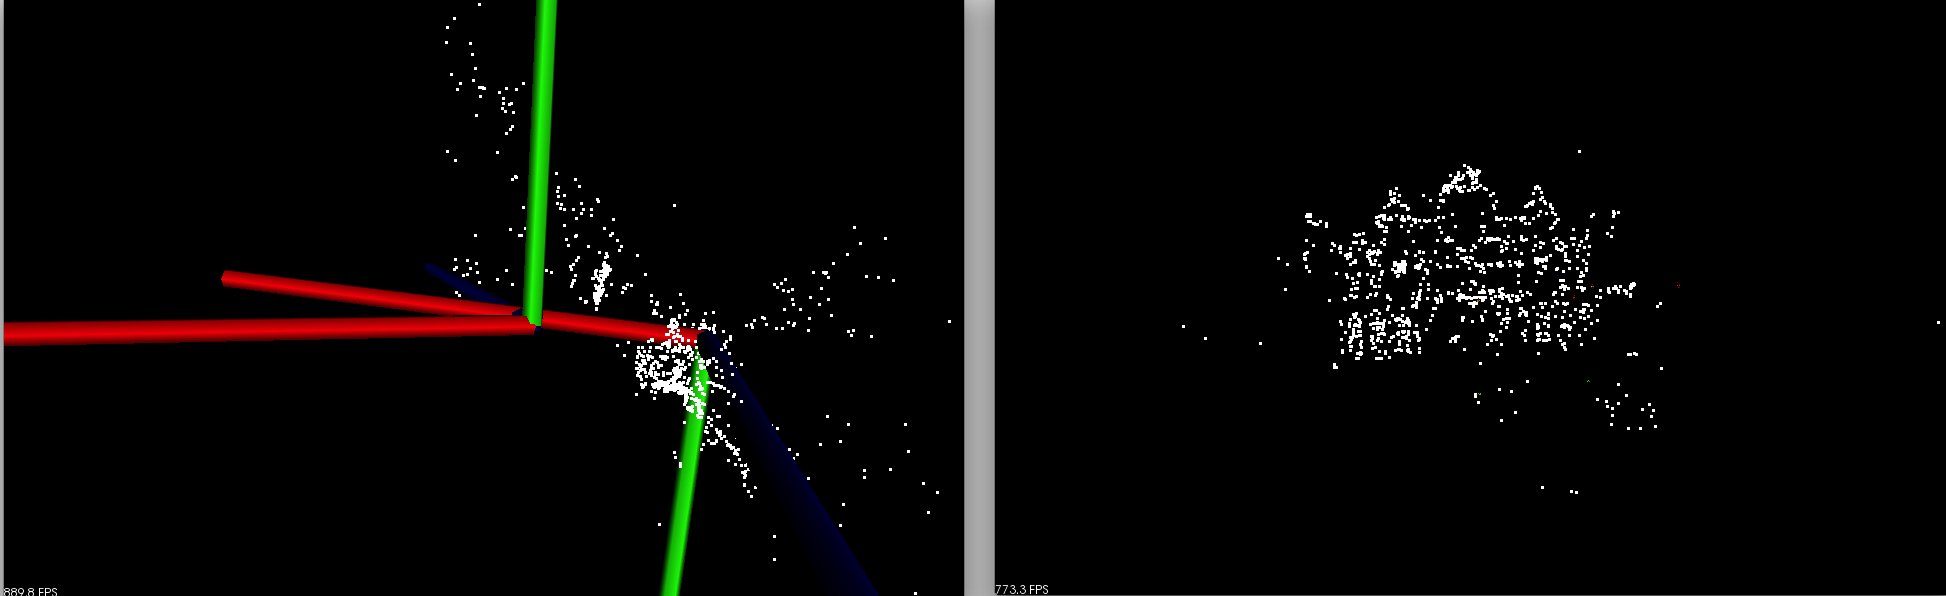
\includegraphics[width=0.9\textwidth]{FailCaseFundamental}
    \caption[Fail test case of Standard 8-point triangulation in comparison to fortunate reconstruction]{Fail test case of Standard 8-point triangulation(left) in comparison to fortunate reconstruction(right)}
    \label{fig:FailCaseFundamental}
\end{figure}
\begin{figure}[p]
    \centering
    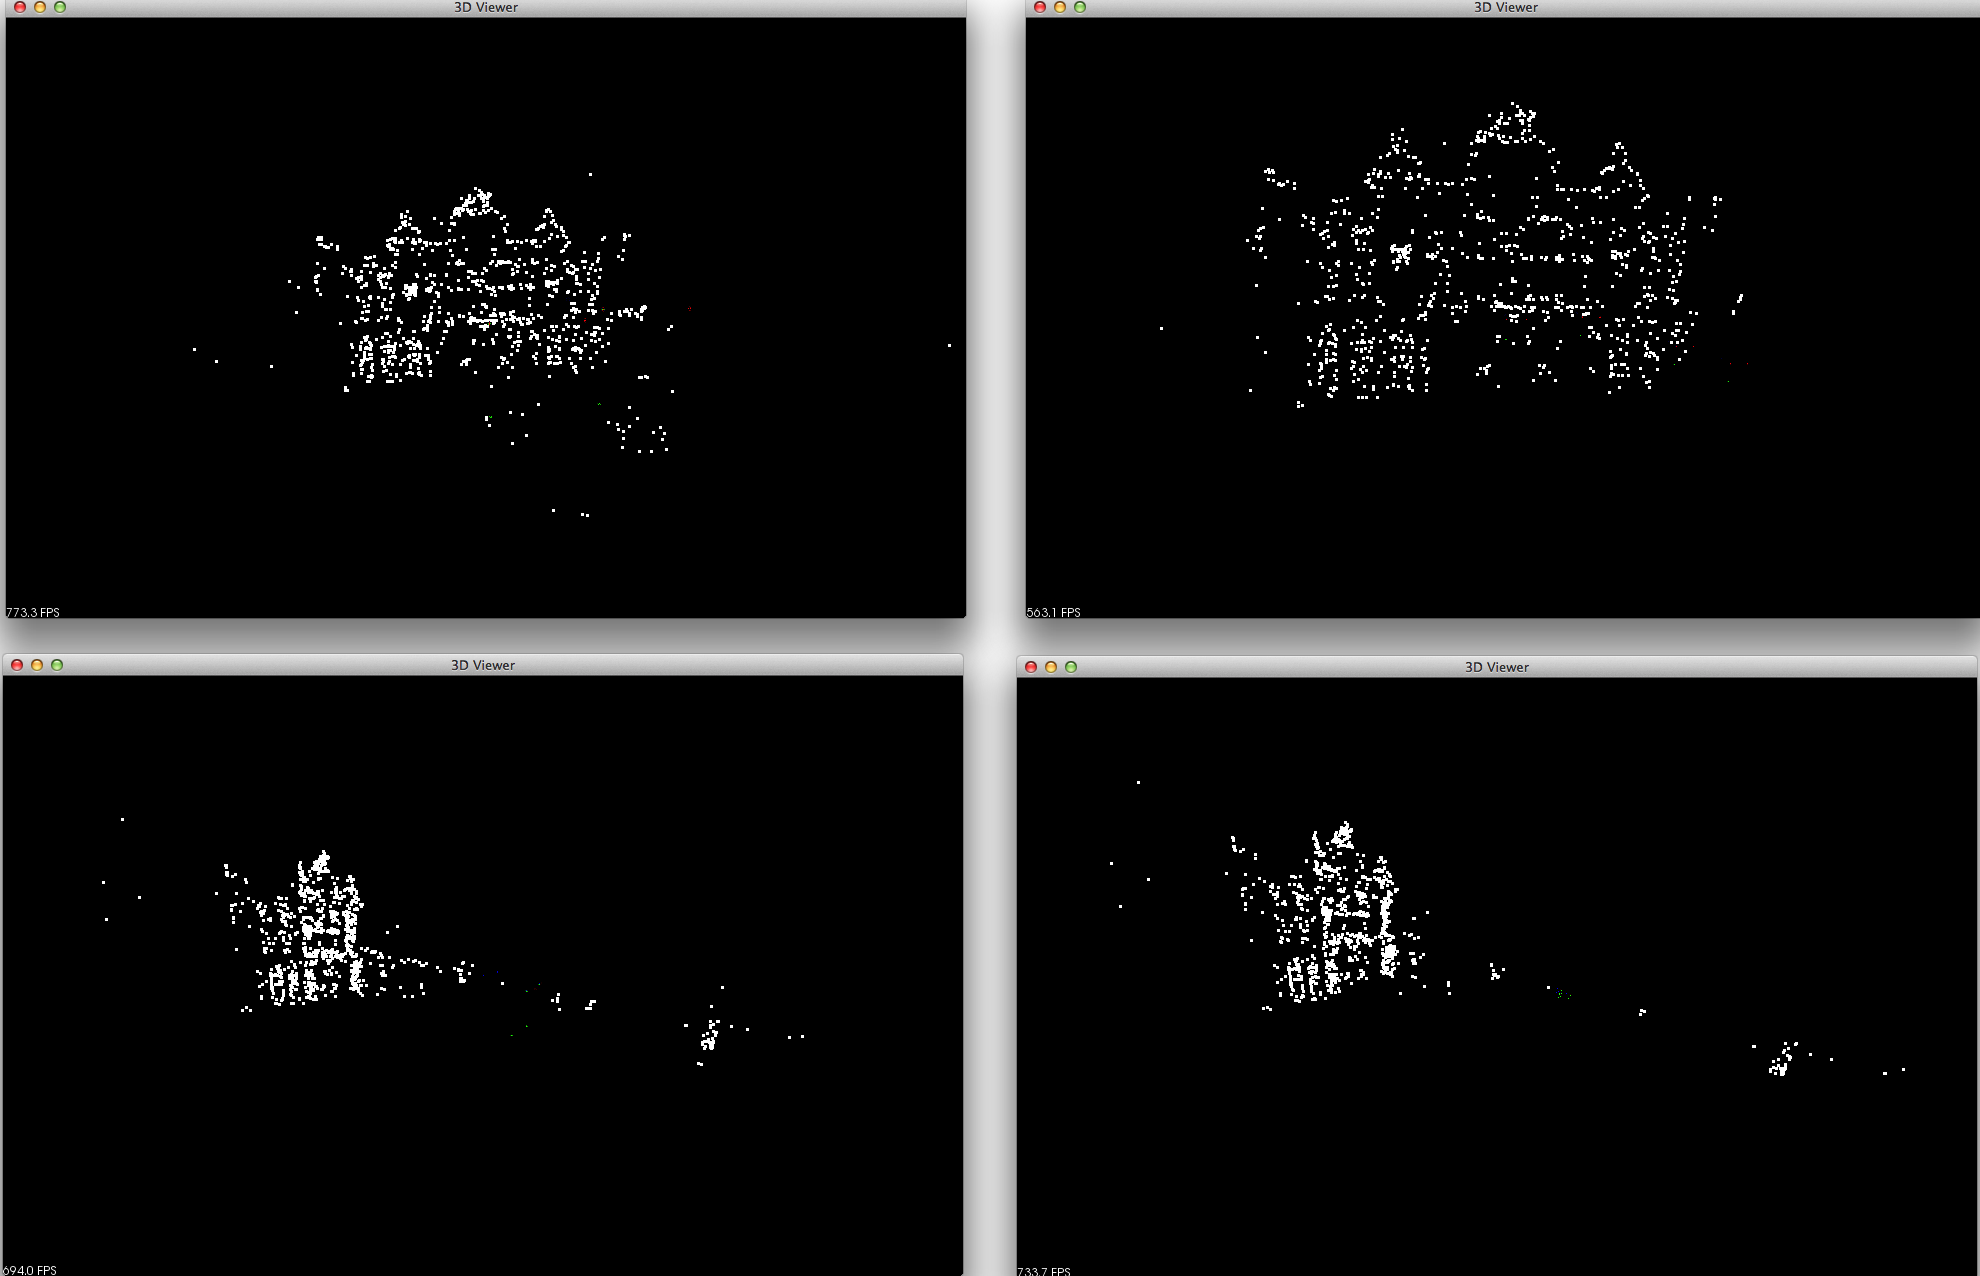
\includegraphics[width=0.9\textwidth]{PoseEstimationMethodComparison}
    \caption[Pose estimation methods comparison]{Pose estimation methods comparison (Views from front and side). Left: Normal Pose Estimation, right: Enhanced Rotation and Translation Pose Estimation. Less outliers appear in the reconstruction if enhancement is applied.}
    \label{fig:PoseEstimationMethodComparison}
\end{figure}
\begin{figure}[p]
    \centering
    \includegraphics[height=18cm]{uniNone4000}
    \caption[Reconstruction results from known translations and rotations from different angles]{Reconstruction results from known translations and rotations from different angles. The upper one shows the front face of building, the others present views from side angles. In the reconstructed model many outliers are present.}
    \label{fig:UniNone4000}
\end{figure}

% ---------------------------------------------------------------------------
% ----------------------- end of thesis sub-document ------------------------
% ---------------------------------------------------------------------------
